\section{Localisation des iles}
Pour localiser les �les, chacune des quatre couleurs est filtr�e et plac�e dans un masque afin d'avoir un traitement individuel. Ensuite, puisque le syst�me poss�de en m�moire les contours des formes qui pourraient repr�senter les �les, celui-ci est en mesure d'identifier la forme qui poss�de le plus haut taux de compatibilit� avec les formes en m�moire.


\section{Localisation du robot}

\section{Alignement du robot}

OUAOUA
%Exemple d'insertion de figure

%\begin{figure}[htp]
%   \centering
%   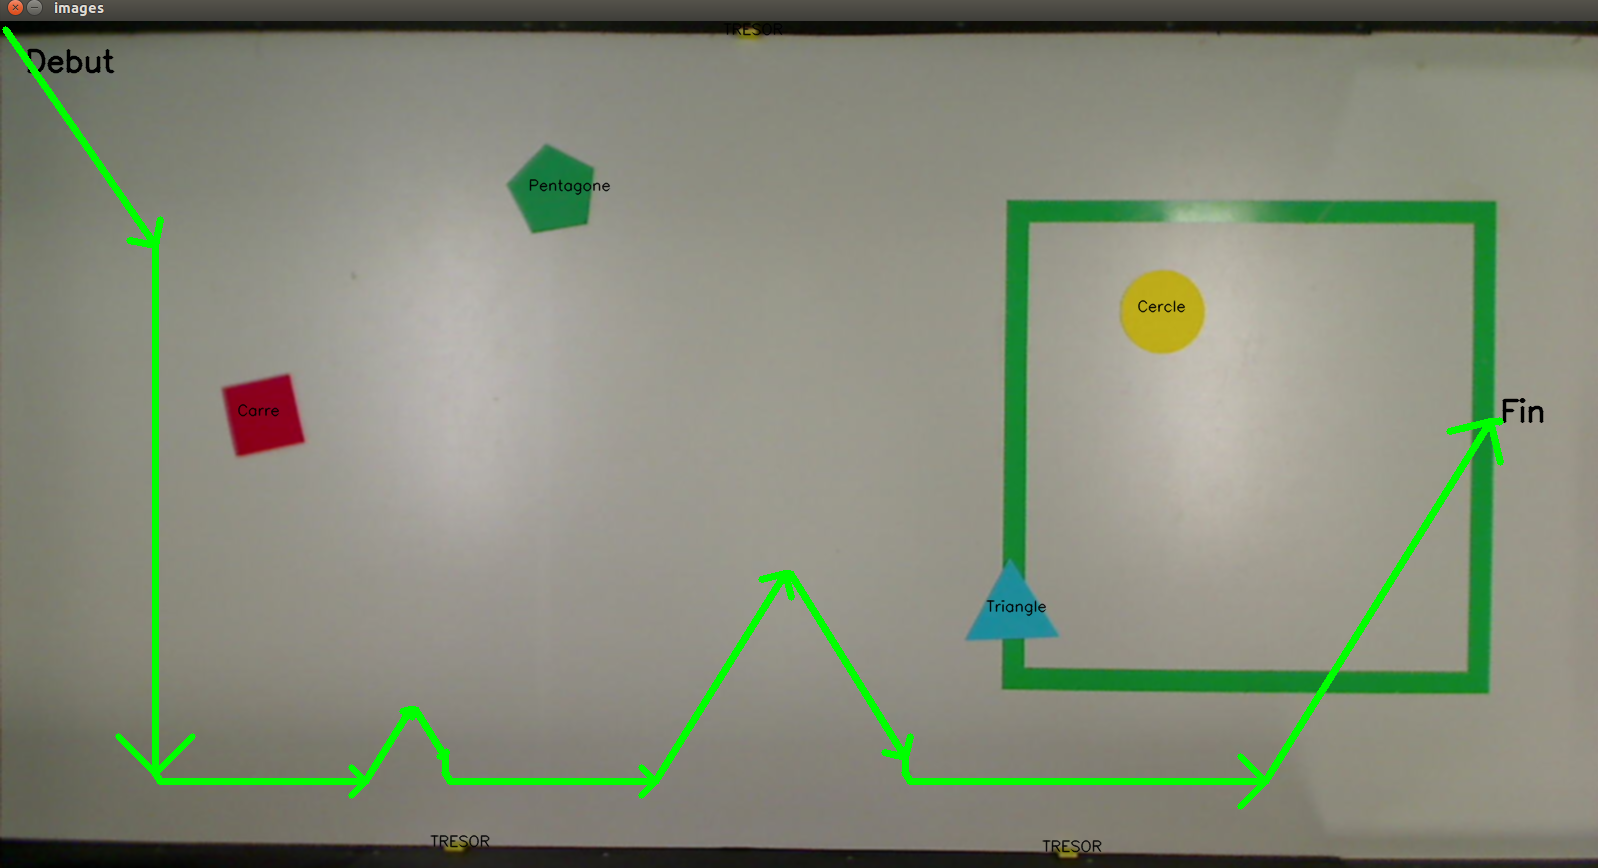
\includegraphics[width=1\textwidth]{fig/trajet.png}
%   \caption{Exemple de trajectoire}
%   \label{f:Trajectoire}
%\end{figure}
%\pagebreak